\pdfminorversion=6
\documentclass[aspectratio=169,10pt]{beamer}

\usepackage[T1]{fontenc}
\usepackage[utf8]{inputenc}
\usepackage{lmodern}
\usepackage{amsmath}
\usepackage{booktabs}
\usepackage{graphicx}
\usepackage{tikz}
\usepackage{qrcode}
\usepackage{pgfplots}
\usepackage{xspace}
\usetikzlibrary{arrows.meta,calc,positioning,fit,decorations.pathreplacing}
\pgfplotsset{compat=1.18}

\definecolor{CornellRed}{HTML}{B31B1B}
\definecolor{CornellDark}{HTML}{222222}
\definecolor{CornellGray}{HTML}{F3F3F1}
\definecolor{Ink}{HTML}{151515}
\definecolor{BlueGray}{HTML}{44616D}
\definecolor{Gold}{HTML}{B68D40}
\definecolor{Green}{HTML}{4C7A5B}
\definecolor{Purple}{HTML}{6B5B95}

\newcommand{\TPHT}{TPHT\xspace}
\newcommand{\Chained}{Chained-TPHT\xspace}
\newcommand{\Flat}{Flattened-TPHT\xspace}
\newcommand{\keyterm}[1]{\textcolor{CornellRed}{\textbf{#1}}}
\newcommand{\metric}[2]{\textcolor{CornellRed}{\textbf{#1}}\hspace{0.35em}{\large #2}}
\newcommand{\apiop}[2]{{\ttfamily #1}\ensuremath{\left(#2\right)}}
\newcommand{\slotball}[3]{%
  \ifnum#3=1
    \fill[Ink] (#1,#2) circle (2.35pt);
  \else
    \draw[Ink,line width=0.55pt,fill=white] (#1,#2) circle (2.35pt);
  \fi
}

\mode<presentation>{
  \usetheme{default}
  \usefonttheme{professionalfonts}
  \useinnertheme{rectangles}
  \setbeamertemplate{navigation symbols}{}
  \setbeamertemplate{blocks}[rounded][shadow=false]
}

\setbeamercolor{normal text}{fg=Ink,bg=white}
\setbeamercolor{frametitle}{fg=white,bg=CornellRed}
\setbeamercolor{title}{fg=white,bg=CornellRed}
\setbeamercolor{subtitle}{fg=white}
\setbeamercolor{author}{fg=white}
\setbeamercolor{date}{fg=white}
\setbeamercolor{block title}{fg=white,bg=CornellRed}
\setbeamercolor{block body}{fg=Ink,bg=CornellGray}
\setbeamercolor{alerted text}{fg=CornellRed}

\setbeamerfont{title}{size=\Large,series=\bfseries}
\setbeamerfont{subtitle}{size=\normalsize}
\setbeamerfont{frametitle}{size=\LARGE,series=\bfseries}
\setbeamerfont{block title}{series=\bfseries}

\setbeamertemplate{frametitle}{
  \nointerlineskip
  \begin{beamercolorbox}[wd=\paperwidth,ht=0.72cm,dp=0.22cm,leftskip=0.55cm,rightskip=0.45cm]{frametitle}
    \usebeamerfont{frametitle}\insertframetitle
    \hfill {\footnotesize Cornell University}
  \end{beamercolorbox}
}

\setbeamertemplate{footline}{
  \leavevmode
  \hbox{
    \begin{beamercolorbox}[wd=.70\paperwidth,ht=2.4ex,dp=1.1ex,leftskip=0.55cm]{normal text}
      {\small Succinct and Fast Tiny Pointer Hash Tables}
    \end{beamercolorbox}
    \begin{beamercolorbox}[wd=.30\paperwidth,ht=2.4ex,dp=1.1ex,rightskip=0.55cm plus 1fil]{normal text}
      \hfill {\scriptsize \insertframenumber/\inserttotalframenumber}
    \end{beamercolorbox}
  }
}

\title{Succinct and Fast Tiny Pointer Hash Tables}
\subtitle{Fast hash tables, without the memory tax}
\author{Xilin Tang \quad Yuqi Mai \quad William Kuszmaul \quad Alex Conway}
\institute{Cornell University \quad Carnegie Mellon University \quad Cornell Tech}
\date{VLDB 2026}

\newcommand{\authorphoto}[5]{%
  \begin{tikzpicture}[baseline=-0.35ex]
    \begin{scope}
      \clip (0,0) circle (0.60cm);
      \node[inner sep=0pt] at (#3,#4) {\includegraphics[height=#2]{#1}};
      \fill[white,opacity=#5] (-0.60cm,-0.60cm) rectangle (0.60cm,0.60cm);
    \end{scope}
    \draw[white,line width=0.8pt] (0,0) circle (0.60cm);
  \end{tikzpicture}%
}

\newcommand{\authorcard}[7]{%
  \begin{minipage}[t]{0.215\paperwidth}
    \centering
    \parbox[t][0.72cm][t]{\linewidth}{\centering
      {\small\bfseries #1}\par
      {\scriptsize\color{white!84}#2}\par
    }
    \vspace{0.12cm}
    \authorphoto{#3}{#4}{#5}{#6}{#7}\par
  \end{minipage}%
}

\newcommand{\titleband}{
  \begin{tikzpicture}[remember picture,overlay]
    \fill[CornellRed] (current page.south west) rectangle (current page.north east);
    \fill[white,opacity=0.10] ($(current page.south west)+(0,0.4)$) rectangle ($(current page.north east)+(0,-6.45)$);
    \draw[white,opacity=0.22,line width=0.8pt] ($(current page.north west)+(0.7,-0.85)$) -- ($(current page.north east)+(-0.7,-0.85)$);
    \node[anchor=north east,white,opacity=0.90] at ($(current page.north east)+(-0.55,-0.35)$) {\small VLDB 2026};
  \end{tikzpicture}
}

\begin{document}

\begin{frame}[plain]
  \titleband
  \vspace{0.88cm}
  \begin{center}
    {\color{white}\resizebox{0.88\paperwidth}{!}{\bfseries\inserttitle}}\par
    \vspace{0.36cm}
    \begin{tikzpicture}
      \node[fill=white,rounded corners=3pt,inner xsep=13pt,inner ysep=7pt,text=CornellRed]
        {\Large\bfseries \insertsubtitle};
    \end{tikzpicture}
  \end{center}
  \vspace{0.35cm}
  \begin{beamercolorbox}[wd=0.94\paperwidth,sep=0.25cm,center]{author}
    \authorcard{Xilin Tang}{Cornell University}{assets/figures/xilin-tang.jpeg}{1.36cm}{0cm}{-0.03cm}{0}
    \hfill
    \authorcard{Yuqi Mai}{Cornell University}{assets/figures/yuqi-mai.jpeg}{3.62cm}{1.17cm}{0.13cm}{0}
    \hfill
    \authorcard{William Kuszmaul}{Carnegie Mellon University}{assets/figures/william-kuszmaul.jpeg}{1.62cm}{-0.04cm}{-0.17cm}{0}
    \hfill
    \authorcard{Alex Conway}{Cornell Tech}{assets/figures/alex-conway.jpeg}{1.72cm}{0.02cm}{-0.13cm}{0}
  \end{beamercolorbox}
\end{frame}

\begin{frame}{Please use our code}
  \vspace{0.18cm}
  \begin{center}
    {\LARGE\bfseries Who can refuse a performance boost}\par
    \vspace{0.12cm}
    {\LARGE\bfseries by just changing their hash table library?}\par
    \vspace{0.22cm}
    {\Large Drop in \href{https://github.com/Xilinion/TPHT}{\keyterm{TPHT}} for faster, smaller dictionaries.}
  \end{center}

  \vspace{0.12cm}
  \begin{center}
  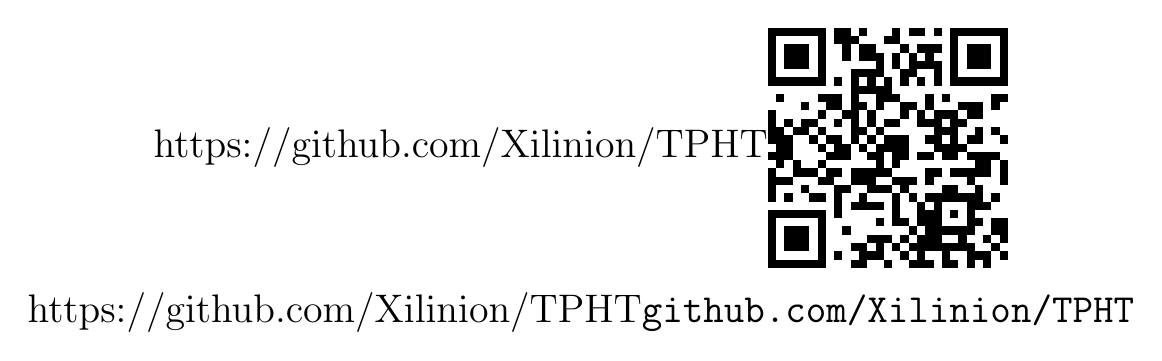
\begin{tikzpicture}[x=1cm,y=1cm,every node/.style={font=\Large}]
    \node[align=center,inner sep=0pt] at (0,0)
      {\href{https://github.com/Xilinion/TPHT}{\qrcode[height=3.05cm]{https://github.com/Xilinion/TPHT}}\\[8pt]
       \href{https://github.com/Xilinion/TPHT}{\texttt{github.com/Xilinion/TPHT}}};
  \end{tikzpicture}
  \end{center}
\end{frame}

\begin{frame}{What is a dictionary?}
  \vspace{0.10cm}
  {\Large A \textbf{dictionary} stores \textcolor{BlueGray}{\textbf{key--value pairs}} and supports updates and lookups.}\par
  \vspace{0.08cm}
  {\small\color{BlueGray} Abstractly: entries are \((k,v)\in K\times V\), and lookup is a partial function \(f:K\to V\cup\{\bot\}\).}\par
  \vspace{0.22cm}
  \begin{center}
  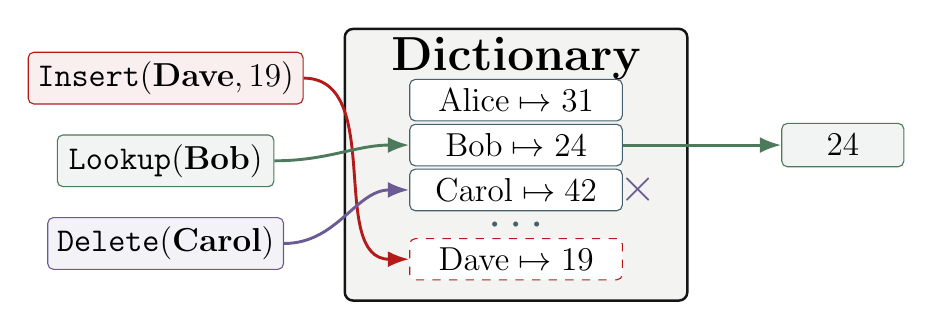
\begin{tikzpicture}[x=1cm,y=1cm]
    \node[draw=Ink,rounded corners=3pt,line width=0.9pt,minimum width=4.35cm,minimum height=3.45cm,fill=CornellGray] (dict) at (0,0) {};
    \node[anchor=north,font=\LARGE\bfseries] at (dict.north) {Dictionary};
    \node[draw=BlueGray,fill=white,rounded corners=2pt,minimum width=2.70cm,minimum height=0.42cm,font=\large] (alice) at (0,0.82) {\(\text{Alice}\mapsto 31\)};
    \node[draw=BlueGray,fill=white,rounded corners=2pt,minimum width=2.70cm,minimum height=0.42cm,font=\large] (bob) at (0,0.25) {\(\text{Bob}\mapsto 24\)};
    \node[draw=BlueGray,fill=white,rounded corners=2pt,minimum width=2.70cm,minimum height=0.42cm,font=\large] (carol) at (0,-0.32) {\(\text{Carol}\mapsto 42\)};
    \node[font=\LARGE\bfseries\color{BlueGray}] at (0,-0.78) {\(\cdots\)};
    \node[draw=CornellRed,dashed,fill=white,rounded corners=2pt,minimum width=2.70cm,minimum height=0.42cm,font=\large] (dave) at (0,-1.20) {\(\text{Dave}\mapsto 19\)};

    \node[draw=CornellRed,fill=CornellRed!7,rounded corners=2pt,minimum width=2.75cm,minimum height=0.55cm,font=\large\bfseries] (insert) at (-4.45,1.10) {\apiop{Insert}{\text{Dave}, 19}};
    \node[draw=Green,fill=Green!8,rounded corners=2pt,minimum width=2.75cm,minimum height=0.55cm,font=\large\bfseries] (lookup) at (-4.45,0.05) {\apiop{Lookup}{\text{Bob}}};
    \node[draw=Purple,fill=Purple!8,rounded corners=2pt,minimum width=2.75cm,minimum height=0.55cm,font=\large\bfseries] (delete) at (-4.45,-1.00) {\apiop{Delete}{\text{Carol}}};

    \draw[-Latex,CornellRed,line width=1.05pt] (insert.east) to[out=0,in=180] (dave.west);
    \draw[-Latex,Green,line width=1.05pt] (lookup.east) to[out=0,in=180] (bob.west);
    \draw[-Latex,Purple,line width=1.05pt] (delete.east) to[out=0,in=180] (carol.west);
    \node[Purple,font=\LARGE\bfseries] at (1.55,-0.32) {\(\times\)};

    \node[draw=Green,fill=Green!8,rounded corners=2pt,minimum width=1.55cm,minimum height=0.55cm,font=\large\bfseries] (value) at (4.15,0.25) {\(24\)};
    \draw[-Latex,Green,line width=1.05pt] (bob.east) to[out=0,in=180] (value.west);
  \end{tikzpicture}
  \end{center}
  \note{
    Begin with the abstract object. A dictionary is the API: it stores key-value pairs. Mathematically, you can think of it as storing pairs from K times V, while lookup is a partial function from keys to values, returning bottom when the key is absent. The main operations are insert, lookup, and delete. This slide should be brief; it is just setting up what a hash table implements.
  }
\end{frame}

\begin{frame}{What is a hash table?}
  \vspace{0.08cm}
  {\Large A \textbf{hash table} is a construction for dictionaries: it uses a \textbf{hash function} to help assign each key--value pair to an array slot.}\par
  \vspace{0.20cm}
  \begin{columns}[T,onlytextwidth]
    \column{0.58\textwidth}
    \begin{center}
    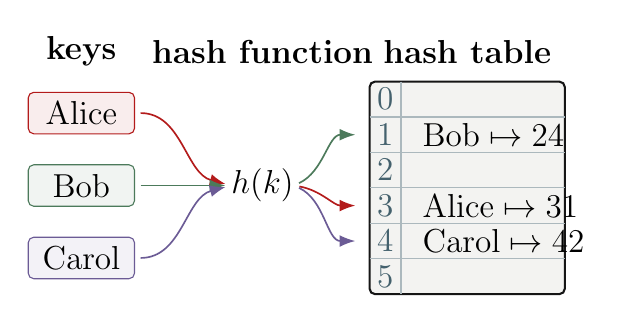
\begin{tikzpicture}[x=1cm,y=1cm,>={Latex[length=1.55mm,width=1.0mm]},every node/.style={font=\large}]
      \node[font=\large\bfseries] at (-3.78,1.80) {keys};
      \node[draw=CornellRed,fill=CornellRed!8,rounded corners=2pt,minimum width=1.35cm,minimum height=0.48cm] (alicekey) at (-3.78,1.02) {Alice};
      \node[draw=Green,fill=Green!8,rounded corners=2pt,minimum width=1.35cm,minimum height=0.48cm] (bobkey) at (-3.78,0.10) {Bob};
      \node[draw=Purple,fill=Purple!8,rounded corners=2pt,minimum width=1.35cm,minimum height=0.48cm] (carolkey) at (-3.78,-0.82) {Carol};

      \node[font=\large\bfseries] at (-1.48,1.80) {hash function};
      \node[font=\large\bfseries] (hash) at (-1.48,0.10) {\(h(k)\)};
      \coordinate (hashL) at (-1.88,0.10);
      \coordinate (hashR) at (-1.08,0.10);

      \node[font=\large\bfseries] at (1.12,1.80) {hash table};
      \draw[draw=Ink,rounded corners=2pt,fill=CornellGray,line width=0.75pt] (-0.12,-1.28) rectangle (2.36,1.42);
      \foreach \j in {1,...,5} {
        \draw[BlueGray!45,line width=0.45pt] (-0.12,{1.42-0.45*\j}) -- (2.36,{1.42-0.45*\j});
      }
      \draw[BlueGray!45,line width=0.55pt] (0.28,1.42) -- (0.28,-1.28);
      \foreach \i in {0,...,5} {
        \node[anchor=center,text=BlueGray] at (0.08,{1.195-0.45*\i}) {\i};
      }
      \node[anchor=west] at (0.43,0.745) {\(\text{Bob}\mapsto 24\)};
      \node[anchor=west] at (0.43,-0.155) {\(\text{Alice}\mapsto 31\)};
      \node[anchor=west] at (0.43,-0.605) {\(\text{Carol}\mapsto 42\)};
      \coordinate (row1target) at (-0.23,0.745);
      \coordinate (row3target) at (-0.23,-0.155);
      \coordinate (row4target) at (-0.23,-0.605);

      \draw[-Latex,CornellRed,line width=0.6pt,shorten >=2pt,shorten <=2pt]
        (alicekey.east) to[out=0,in=165] (hashL);
      \draw[-Latex,Green,line width=0.6pt,shorten >=2pt,shorten <=2pt]
        (bobkey.east) -- (hashL);
      \draw[-Latex,Purple,line width=0.6pt,shorten >=2pt,shorten <=2pt]
        (carolkey.east) to[out=0,in=195] (hashL);

      \draw[-Latex,CornellRed,line width=0.6pt,shorten >=2pt,shorten <=2pt]
        (hashR) to[out=-10,in=180] (row3target);
      \draw[-Latex,Green,line width=0.6pt,shorten >=2pt,shorten <=2pt]
        (hashR) to[out=25,in=180] (row1target);
      \draw[-Latex,Purple,line width=0.6pt,shorten >=2pt,shorten <=2pt]
        (hashR) to[out=-25,in=180] (row4target);
    \end{tikzpicture}
    \end{center}

    \column{0.39\textwidth}
    \vspace{0.08cm}
    \begin{minipage}{\linewidth}
    \raggedright
    {\large\bfseries Hashing dates to \keyterm{1953}}\par
    \vspace{0.16cm}
    {\large Expected \(O(1)\) operations}\par
    \vspace{0.12cm}
    {\large Linear probing, chaining, \(\ldots\)}\par
    \vspace{0.22cm}
    {\large Decades of tuning for
    \(\left\{\begin{array}{l}
      \text{\textbf{speed}}\\[-1pt]
      \text{\textbf{space}}
    \end{array}\right.\)}
    \end{minipage}

    \vspace{0.28cm}
    \noindent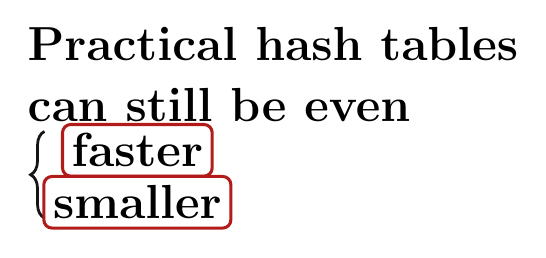
\begin{tikzpicture}[x=1cm,y=1cm]
      \node[anchor=west,align=left,font=\LARGE\bfseries,inner sep=0pt] (theme) at (0,0.92)
        {Practical hash tables\\can still be even};
      \draw[decorate,decoration={brace,amplitude=5pt},line width=1pt,Ink]
        (0.22,-0.90) -- (0.22,0.20);
      \node[draw=CornellRed,line width=1.1pt,rounded corners=3pt,minimum width=1.72cm,minimum height=0.48cm,font=\LARGE\bfseries] at (1.40,-0.04)
        {faster};
      \node[draw=CornellRed,line width=1.1pt,rounded corners=3pt,minimum width=1.72cm,minimum height=0.48cm,font=\LARGE\bfseries] at (1.40,-0.70)
        {smaller};
    \end{tikzpicture}
  \end{columns}
  \note{
    Now reveal the concrete implementation. Hash tables are a construction for the dictionary API: they use a hash function to help decide where a key-value pair belongs in an array. Different tables use that hash information differently--linear probing, chaining, and many other designs--so this slide intentionally leaves some space there. Historically this dates to 1953 and promises O(1) operations, so it is tempting to say: done. But even after many implementations and decades of optimization for speed and space, this work argues that practical hash tables can still be even faster and smaller.
  }
\end{frame}

\begin{frame}{Secret Sauce}
  \begin{columns}[T,onlytextwidth]
    \column{0.39\textwidth}
      \vspace{0.20cm}
      {\LARGE\bfseries Three ingredients:}\par
      \vspace{0.16cm}
      \begin{enumerate}\Large
        \item \keyterm{Tiny pointers}\\
          {\large compress the \textbf{pointer}}
          \vspace{0.14cm}
        \item \keyterm{Quotienting}\\
          {\large compress the \textbf{key}}
          \vspace{0.14cm}
        \item \keyterm{Cache-friendly layout}\\
          {\large compress the \textbf{execution time}}
      \end{enumerate}

    \column{0.58\textwidth}
      \begin{center}
        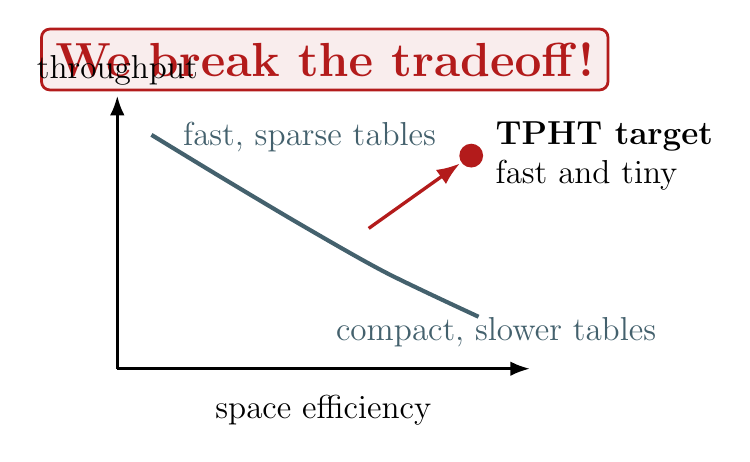
\begin{tikzpicture}[x=0.62cm,y=0.66cm]
          \node[draw=CornellRed,fill=CornellRed!8,line width=1.0pt,rounded corners=3pt,
                align=center,font=\LARGE\bfseries,text=CornellRed,inner sep=5pt]
                at (4.25,5.95) {We break the tradeoff!};
          \draw[-Latex,line width=0.9pt] (0,0) -- (8.45,0);
          \node[font=\large,anchor=north] at (4.22,-0.32) {space efficiency};
          \draw[-Latex,line width=0.9pt] (0,0) -- (0,5.25) node[above,font=\large] {throughput};
          \draw[BlueGray,line width=1.5pt] plot[smooth] coordinates {(0.7,4.5) (2.1,3.7) (3.8,2.75) (5.5,1.85) (7.4,1.0)};
          \node[BlueGray,anchor=west,font=\large] at (1.15,4.45) {fast, sparse tables};
          \node[BlueGray,anchor=west,font=\large] at (4.28,0.70) {compact, slower tables};
          \fill[CornellRed] (7.25,4.1) circle (4.3pt);
          \node[align=left,anchor=west,font=\large] at (7.55,4.1) {\textbf{TPHT target}\\fast and tiny};
          \draw[CornellRed,very thick,-Latex] (5.15,2.7) -- (7.02,3.95);
        \end{tikzpicture}
      \end{center}
  \end{columns}
\end{frame}

\begin{frame}{Ingredient 1: Tiny Pointer}
  \vspace{0.05cm}
  {\Large A \keyterm{tiny pointer} is a \textbf{very short pointer} that can be decoded only with its \textbf{owner}.}

  \vspace{0.14cm}
  \begin{center}
  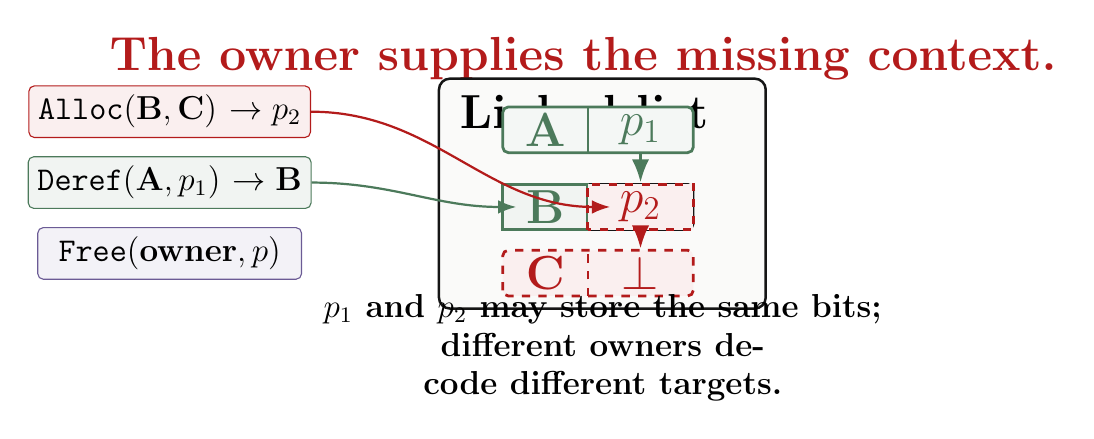
\begin{tikzpicture}[x=1cm,y=1cm,>=Latex,every node/.style={font=\large}]
    \node[align=center,font=\LARGE\bfseries,text=CornellRed] at (0.80,3.38)
      {The owner supplies the missing context.};

    \node[draw=CornellRed,fill=CornellRed!7,rounded corners=2pt,minimum width=3.35cm,minimum height=0.55cm,font=\large\bfseries] (alloc) at (-4.45,2.70)
      {\apiop{Alloc}{\text{B}, \text{C}} \(\to p_2\)};
    \node[draw=Green,fill=Green!8,rounded corners=2pt,minimum width=3.35cm,minimum height=0.55cm,font=\large\bfseries] (deref) at (-4.45,1.80)
      {\apiop{Deref}{\text{A}, p_1} \(\to \text{B}\)};
    \node[draw=Purple,fill=Purple!8,rounded corners=2pt,minimum width=3.35cm,minimum height=0.55cm,font=\large\bfseries] (free) at (-4.45,0.90)
      {\apiop{Free}{\text{owner}, p}};

    \draw[Ink,line width=0.9pt,rounded corners=4pt,fill=CornellGray!45] (-1.03,0.20) rectangle (3.12,3.12);
    \node[anchor=north west,font=\LARGE\bfseries] at (-0.89,3.03) {Linked list};

    \draw[Green,line width=1.0pt,rounded corners=2pt,fill=Green!6] (-0.22,2.18) rectangle (2.20,2.76);
    \draw[Green,line width=0.8pt] (0.86,2.18) -- (0.86,2.76);
    \node[Green,font=\LARGE\bfseries] (aobj) at (0.32,2.47) {A};
    \node[Green,font=\LARGE\bfseries] (aptr) at (1.53,2.47) {\(p_1\)};

    \draw[Ink,line width=0.8pt,rounded corners=2pt,fill=white] (-0.22,1.20) rectangle (2.20,1.78);
    \draw[Green,line width=1.0pt,fill=Green!8] (-0.22,1.20) rectangle (0.86,1.78);
    \draw[CornellRed,dashed,line width=1.0pt,fill=CornellRed!7] (0.86,1.20) rectangle (2.20,1.78);
    \node[Green,font=\LARGE\bfseries] (bobj) at (0.32,1.49) {B};
    \node[CornellRed,font=\LARGE\bfseries] (bptr) at (1.53,1.49) {\(p_2\)};

    \draw[CornellRed,dashed,line width=1.0pt,rounded corners=2pt,fill=CornellRed!7] (-0.22,0.36) rectangle (2.20,0.94);
    \draw[CornellRed,dashed,line width=0.8pt] (0.86,0.36) -- (0.86,0.94);
    \node[CornellRed,font=\LARGE\bfseries] (cobj) at (0.32,0.65) {C};
    \node[CornellRed,font=\LARGE\bfseries] (cptr) at (1.53,0.65) {\(\bot\)};

    \draw[-Latex,very thick,Green] (1.53,2.18) -- (1.53,1.80);
    \draw[-Latex,very thick,CornellRed,dashed] (1.53,1.20) -- (1.53,0.96);

    \draw[-Latex,Green,thick] (deref.east) to[out=0,in=180] (bobj.west);
    \draw[-Latex,CornellRed,thick] (alloc.east) to[out=0,in=180] (bptr.west);

    \node[align=center,text width=8.1cm,font=\large\bfseries] at (1.05,-0.30)
      {\(p_1\) and \(p_2\) may store the same bits;\\different owners decode different targets.};
  \end{tikzpicture}
  \end{center}
\end{frame}

\begin{frame}{Tiny Pointer: Implementation}
  \vspace{0.04cm}
  {\Large Tiny pointers require a \keyterm{special memory allocator}, called a \textbf{dereference table} in our literature.}

  \vspace{0.05cm}
  \begin{center}
  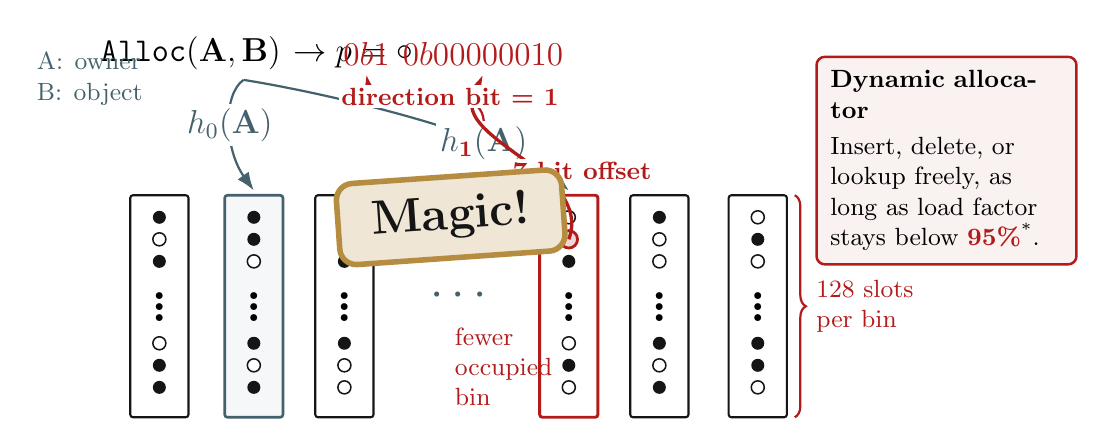
\begin{tikzpicture}[x=1cm,y=1cm,>=Latex,every node/.style={font=\large}]
    \node[font=\large\bfseries] (api) at (-3.98,3.70)
      {\apiop{Alloc}{\text{A}, \text{B}} \(\to p =\)};
    \node[anchor=east,align=left,font=\small,BlueGray] at (-5.14,3.38)
      {\(\text{A}\): owner\\\(\text{B}\): object};
    \node[font=\large\bfseries,text=CornellRed] (dirbit) at (-2.42,3.70) {\(0b1\)};
    \node[font=\large\bfseries] (concat) at (-1.93,3.70) {\(\circ\)};
    \node[font=\large\bfseries,text=CornellRed] (offsetbits) at (-0.94,3.70) {\(0b00000010\)};
    \node[font=\LARGE\bfseries,BlueGray] at (-1.25,0.62) {\(\cdots\)};

    \foreach \x in {-5.05,-2.70,1.30,2.55} {
      \draw[Ink,line width=0.75pt,rounded corners=1pt,fill=white] ({\x-0.37},-0.92) rectangle +(0.74,2.82);
    }

    \draw[BlueGray,line width=0.95pt,rounded corners=1pt,fill=BlueGray!5] (-4.22,-0.92) rectangle +(0.74,2.82);

    \draw[CornellRed,line width=1.05pt,rounded corners=1pt,fill=white] (-0.22,-0.92) rectangle +(0.74,2.82);

    \slotball{-5.05}{1.62}{1}
    \slotball{-5.05}{1.34}{0}
    \slotball{-5.05}{1.06}{1}
    \node[font=\LARGE\bfseries] at (-5.05,0.58) {\(\vdots\)};
    \slotball{-5.05}{0.02}{0}
    \slotball{-5.05}{-0.26}{1}
    \slotball{-5.05}{-0.54}{1}

    \slotball{-3.85}{1.62}{1}
    \slotball{-3.85}{1.34}{1}
    \slotball{-3.85}{1.06}{0}
    \node[font=\LARGE\bfseries] at (-3.85,0.58) {\(\vdots\)};
    \slotball{-3.85}{0.02}{1}
    \slotball{-3.85}{-0.26}{0}
    \slotball{-3.85}{-0.54}{1}

    \slotball{-2.70}{1.62}{0}
    \slotball{-2.70}{1.34}{1}
    \slotball{-2.70}{1.06}{1}
    \node[font=\LARGE\bfseries] at (-2.70,0.58) {\(\vdots\)};
    \slotball{-2.70}{0.02}{1}
    \slotball{-2.70}{-0.26}{0}
    \slotball{-2.70}{-0.54}{0}

    \slotball{0.15}{1.62}{0}
    \draw[CornellRed,line width=1.0pt,fill=CornellRed!18] (0.15,1.34) circle (3.15pt);
    \coordinate (slot) at (0.15,1.34);
    \slotball{0.15}{1.06}{1}
    \node[font=\LARGE\bfseries] at (0.15,0.58) {\(\vdots\)};
    \slotball{0.15}{0.02}{0}
    \slotball{0.15}{-0.26}{1}
    \slotball{0.15}{-0.54}{0}

    \slotball{1.30}{1.62}{1}
    \slotball{1.30}{1.34}{0}
    \slotball{1.30}{1.06}{0}
    \node[font=\LARGE\bfseries] at (1.30,0.58) {\(\vdots\)};
    \slotball{1.30}{0.02}{1}
    \slotball{1.30}{-0.26}{0}
    \slotball{1.30}{-0.54}{1}

    \slotball{2.55}{1.62}{0}
    \slotball{2.55}{1.34}{1}
    \slotball{2.55}{1.06}{0}
    \node[font=\LARGE\bfseries] at (2.55,0.58) {\(\vdots\)};
    \slotball{2.55}{0.02}{1}
    \slotball{2.55}{-0.26}{1}
    \slotball{2.55}{-0.54}{0}

    \draw[-Latex,BlueGray,thick]
      (api.south) .. controls (-4.25,3.18) and (-4.22,2.48) ..
      node[pos=0.50,fill=white,inner sep=1.6pt,font=\large\bfseries] (h0) {\(h_0(\text{A})\)}
      (-3.85,1.96);
    \draw[-Latex,BlueGray,thick]
      (api.south) .. controls (-2.82,3.18) and (-0.58,2.64) ..
      node[pos=0.68,fill=white,inner sep=1.6pt,font=\large\bfseries] (h1) {\(h_{\textcolor{CornellRed}{\mathbf{1}}}(\text{A})\)}
      (0.15,1.96);
    \node[align=left,font=\small,text=CornellRed,anchor=west] at (-1.42,-0.28) {fewer\\occupied\\bin};

    \draw[decorate,decoration={brace,amplitude=4pt},CornellRed,line width=0.8pt] (3.02,1.90) -- (3.02,-0.92);
    \node[anchor=west,align=left,font=\small,text=CornellRed] at (3.17,0.49) {128 slots\\per bin};

    \draw[-Latex,CornellRed,very thick] (slot) to[out=70,in=-115] (offsetbits.south);
    \node[fill=white,inner sep=1pt,font=\small\bfseries,text=CornellRed] at (0.32,2.21) {7-bit offset};
    \draw[-Latex,CornellRed,thick] (h1.north) to[out=95,in=-80] (dirbit.south);
    \node[fill=white,inner sep=1pt,font=\small\bfseries,text=CornellRed] at (-1.36,3.15) {direction bit = 1};

    \node[draw=CornellRed,fill=CornellRed!6,line width=0.9pt,rounded corners=3pt,
          anchor=west,align=left,text width=2.95cm,inner sep=5pt,font=\small]
          at (3.28,2.34)
          {\textbf{Dynamic allocator}\\[2pt]
           Insert, delete, or lookup freely, as long as load factor stays below \textcolor{CornellRed}{\textbf{95\%}}\textsuperscript{*}.};

    \node[draw=Gold,fill=Gold!22,line width=2.0pt,rounded corners=6pt,
          inner xsep=12pt,inner ysep=7pt,font=\LARGE\bfseries,text=Ink,rotate=4]
          at (-1.35,1.62) {Magic!};
  \end{tikzpicture}
  \end{center}
  \vspace{-0.16cm}
  {\small\textsuperscript{*}No strict theoretical promise; empirically supports \(\mathrm{poly}(n)\) operations for \(n<2^{64}\).}
\end{frame}

\begin{frame}{Ingredient 2: Quotienting}
  \vspace{0.05cm}
  {\Large \keyterm{Quotienting} reduces the bits needed to represent a \textbf{key set} by \textbf{partitioning} it.}

  \vspace{0.08cm}
  {\Large Insight: the \textbf{location of a partition} already encodes part of the information.}

  \vspace{0.10cm}
  \begin{center}
  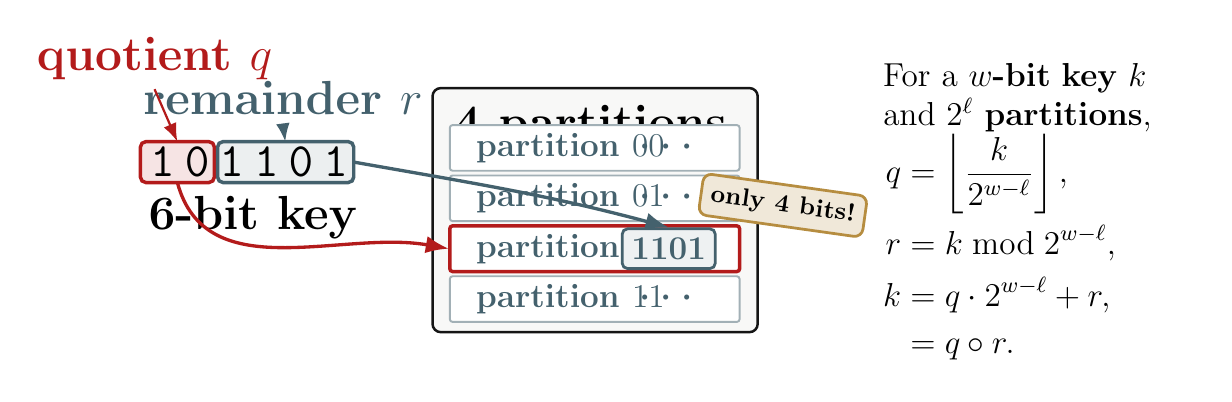
\begin{tikzpicture}[x=1cm,y=1cm,>=Latex,every node/.style={font=\large}]
    \node[anchor=west,font=\LARGE\bfseries] at (-5.68,1.28) {6-bit key};

    \draw[CornellRed,line width=1.25pt,rounded corners=2pt,fill=CornellRed!12]
      (-5.66,1.72) rectangle (-4.72,2.24);
    \draw[BlueGray,line width=1.25pt,rounded corners=2pt,fill=BlueGray!10]
      (-4.68,1.72) rectangle (-2.95,2.24);

    \foreach \b/\x/\name in {1/-5.38/b0,0/-4.94/b1,1/-4.50/b2,1/-4.06/b3,0/-3.62/b4,1/-3.18/b5} {
      \node[font=\LARGE\bfseries\ttfamily,inner sep=1.0pt] (\name) at (\x,1.98) {\b};
    }

    \coordinate (qframe-bottom) at (-5.19,1.72);
    \coordinate (rframe-east) at (-2.95,1.98);
    \coordinate (qframe-north) at (-5.19,2.24);
    \coordinate (rframe-north) at (-3.82,2.24);
    \node[text=CornellRed,font=\LARGE\bfseries] (qlabel) at (-5.48,3.30) {quotient \(q\)};
    \node[text=BlueGray,font=\LARGE\bfseries] (rlabel) at (-3.85,2.80) {remainder \(r\)};
    \draw[-Latex,CornellRed,thick] (qlabel.south) -- (qframe-north);
    \draw[-Latex,BlueGray,thick] (rlabel.south) -- (rframe-north);

    \draw[Ink,line width=0.9pt,rounded corners=3pt,fill=CornellGray!60] (-1.95,-0.18) rectangle (2.18,2.92);
    \node[anchor=north west,font=\LARGE\bfseries] at (-1.80,2.82) {4 partitions};
    \foreach \q/\y in {00/2.16,01/1.52,10/0.88,11/0.24} {
      \draw[BlueGray!50,line width=0.7pt,fill=white,rounded corners=1pt] (-1.73,\y-0.29) rectangle (1.95,\y+0.29);
      \node[anchor=west,font=\large\bfseries,text=BlueGray] at (-1.52,\y) {partition \(\q\)};
    }
    \draw[CornellRed,line width=1.25pt,rounded corners=1pt] (-1.73,0.59) rectangle (1.95,1.17);
    \node[font=\LARGE\bfseries,BlueGray] at (1.02,2.16) {\(\cdots\)};
    \node[font=\LARGE\bfseries,BlueGray] at (1.02,1.52) {\(\cdots\)};
    \node[font=\LARGE\bfseries,BlueGray] at (1.02,0.24) {\(\cdots\)};
    \node[draw=BlueGray,fill=BlueGray!9,line width=1.0pt,rounded corners=2pt,text=BlueGray,
          minimum width=1.05cm,minimum height=0.32cm,font=\large\bfseries] (stored) at (1.05,0.88) {1101};
    \node[draw=Gold,fill=Gold!20,line width=1.0pt,rounded corners=3pt,
          inner sep=3.5pt,font=\small\bfseries,rotate=-8] at (2.5,1.43) {only 4 bits!};

    \draw[-Latex,CornellRed,very thick] (qframe-bottom) to[out=-75,in=170] (-1.74,0.88);
    \draw[-Latex,BlueGray,very thick] (rframe-east) to[out=-10,in=165] (stored.north);

    \node[anchor=west,align=left,text width=3.95cm,font=\large]
          at (3.65,1.32)
          {For a \textbf{\(w\)-bit key} \(k\) and \textbf{\(2^\ell\) partitions},
           \(\begin{aligned}
             q&=\left\lfloor\frac{k}{2^{w-\ell}}\right\rfloor,\\
             r&=k\bmod 2^{w-\ell},\\
             k&=q\cdot 2^{w-\ell}+r,\\
              &=q\circ r.
           \end{aligned}\)};
  \end{tikzpicture}
  \end{center}
  \note{For the talk track: We split the key into two parts. We call the prefix the quotient, and we call the remaining bits the remainder. Since the quotient decides which partition the key belongs to, the partition location itself already remembers those quotient bits; inside the partition we only store the remainder.}
\end{frame}

\begin{frame}{Chained-TPHT}
  \vspace{0.04cm}
  {\Large Let's construct a \keyterm{chained hash table} with our ingredients!}

  \vspace{0.10cm}
  \begin{center}
  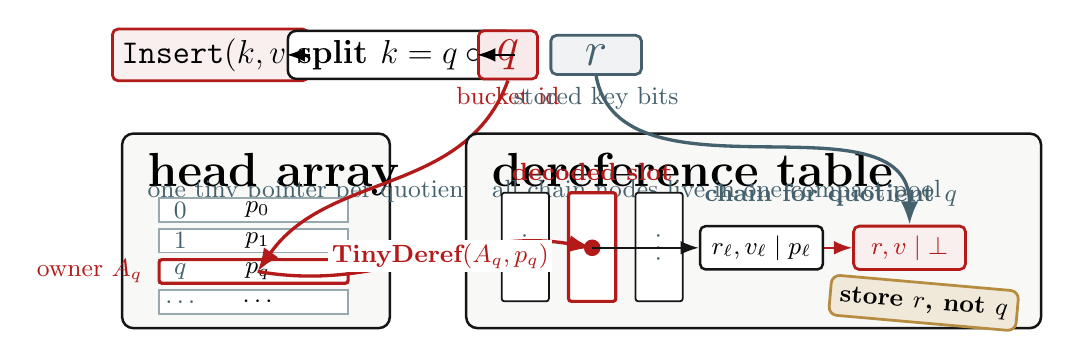
\begin{tikzpicture}[x=1cm,y=1cm,>=Latex,every node/.style={font=\large}]
    \node[draw=CornellRed,fill=CornellRed!7,rounded corners=2pt,line width=1.0pt,
          minimum width=2.25cm,minimum height=0.55cm,font=\large\bfseries] (insert) at (-4.80,2.55)
          {\apiop{Insert}{k,v}};

    \node[draw=Ink,fill=white,line width=0.9pt,rounded corners=3pt,
          minimum width=2.25cm,minimum height=0.55cm,font=\large\bfseries] (split) at (-2.38,2.55)
          {split \(k=q\circ r\)};
    \draw[-Latex,thick] (insert.east) -- (split.west);

    \node[draw=CornellRed,fill=CornellRed!9,line width=1.0pt,rounded corners=2pt,
          minimum width=0.75cm,minimum height=0.47cm,font=\LARGE\bfseries,text=CornellRed] (qbits) at (-1.02,2.55) {\(q\)};
    \node[draw=BlueGray,fill=BlueGray!8,line width=1.0pt,rounded corners=2pt,
          minimum width=1.15cm,minimum height=0.47cm,font=\LARGE\bfseries,text=BlueGray] (rbits) at (0.10,2.55) {\(r\)};
    \draw[-Latex,thick] (split.east) -- (qbits.west);
    \node[anchor=north,font=\small,text=CornellRed] at (-1.02,2.27) {bucket id};
    \node[anchor=north,font=\small,text=BlueGray] at (0.10,2.27) {stored key bits};

    \draw[Ink,line width=0.9pt,rounded corners=4pt,fill=CornellGray!55] (-5.92,-0.92) rectangle (-2.52,1.55);
    \node[anchor=north west,font=\LARGE\bfseries] at (-5.72,1.43) {head array};
    \node[anchor=north west,font=\small,text=BlueGray] at (-5.72,1.08) {one tiny pointer per quotient group};
    \foreach \idx/\val/\y in {0/\(p_0\)/0.58,1/\(p_1\)/0.19,q/\(p_q\)/-0.20,\ldots/\(\cdots\)/-0.59} {
      \draw[BlueGray!55,line width=0.65pt,fill=white] (-5.45,\y-0.15) rectangle (-3.05,\y+0.15);
      \node[font=\small,text=BlueGray] at (-5.18,\y) {\(\idx\)};
      \node[font=\small\bfseries] at (-4.20,\y) {\val};
    }
    \draw[CornellRed,line width=1.15pt,rounded corners=1pt] (-5.45,-0.35) rectangle (-3.05,-0.05);
    \node[font=\small,text=CornellRed,anchor=east] (owner) at (-5.54,-0.20) {owner \(A_q\)};
    \coordinate (headslot) at (-4.20,-0.20);
    \draw[-Latex,CornellRed,very thick] (qbits.south) to[out=-110,in=55] (headslot);

    \draw[Ink,line width=0.9pt,rounded corners=4pt,fill=CornellGray!55] (-1.55,-0.92) rectangle (5.75,1.55);
    \node[anchor=north west,font=\LARGE\bfseries] at (-1.35,1.43) {dereference table};
    \node[anchor=north west,font=\small,text=BlueGray] at (-1.35,1.08) {all chain nodes live in one compact pool};

    \foreach \x/\lab in {-0.80/\(\cdots\),0.05/\(\mathrm{bin}\),0.90/\(\cdots\)} {
      \draw[Ink,line width=0.65pt,rounded corners=1pt,fill=white] (\x-0.30,-0.58) rectangle (\x+0.30,0.80);
      \node[font=\small,text=BlueGray,rotate=90] at (\x,0.10) {\lab};
    }
    \draw[CornellRed,line width=1.15pt,rounded corners=1pt,fill=white] (-0.25,-0.58) rectangle (0.35,0.80);
    \coordinate (slot) at (0.05,0.10);
    \fill[CornellRed] (slot) circle (3.0pt);
    \node[anchor=south,font=\small\bfseries,text=CornellRed] at (0.05,0.83) {decoded slot};
    \draw[-Latex,CornellRed,very thick] (headslot) to[out=-10,in=170]
      node[pos=0.55,fill=white,inner sep=1.3pt,font=\small\bfseries,text=CornellRed]
      {TinyDeref\((A_q,p_q)\)} (slot);

    \node[draw=Ink,fill=white,line width=0.9pt,rounded corners=2pt,
          minimum width=1.56cm,minimum height=0.48cm,font=\small\bfseries] (oldnode) at (2.20,0.10)
          {\(r_\ell,v_\ell\;|\;p_\ell\)};
    \node[draw=CornellRed,fill=CornellRed!7,line width=1.0pt,rounded corners=2pt,
          minimum width=1.42cm,minimum height=0.48cm,font=\small\bfseries,text=CornellRed] (newnode) at (4.08,0.10)
          {\(r,v\;|\;\bot\)};
    \draw[-Latex,Ink,thick] (slot) -- (oldnode.west);
    \draw[-Latex,CornellRed,thick] (oldnode.east) -- (newnode.west);
    \node[anchor=south,font=\small\bfseries,text=BlueGray] at (3.08,0.50)
      {chain for quotient \(q\)};

    \draw[-Latex,BlueGray,very thick] (rbits.south) to[out=-80,in=90] (newnode.north);
    \node[draw=Gold,fill=Gold!20,line width=1.0pt,rounded corners=3pt,
          inner sep=3.5pt,font=\small\bfseries,rotate=-5] at (4.26,-0.60)
          {store \(r\), not \(q\)};
  \end{tikzpicture}
  \end{center}
  \note{This slide moves from the quotienting ingredient to the first full design. Insert splits the key into quotient q and remainder r. The quotient indexes the head array. The head cell stores a tiny pointer, whose owner is the address of that head cell. Dereferencing finds the chain node in the monolithic dereference table. The chain stores only remainders and values, because the quotient is already represented by the head-array location.}
\end{frame}

\begin{frame}{Making TPHT Fast}
  \vspace{0.04cm}
  {\Large \Chained is already \keyterm{more cache-friendly} than normal chaining.}

  \vspace{0.10cm}
  \begin{center}
  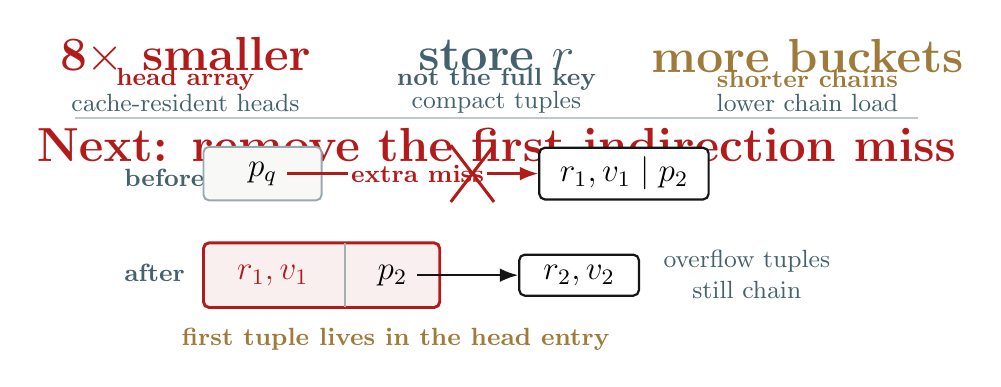
\begin{tikzpicture}[x=1cm,y=1cm,>=Latex,every node/.style={font=\large}]
    \node[align=center,text=CornellRed,font=\LARGE\bfseries] at (-3.95,1.48)
      {8\(\times\) smaller};
    \node[align=center,text=CornellRed,font=\small\bfseries] at (-3.95,1.18)
      {head array};
    \node[align=center,text=BlueGray,font=\LARGE\bfseries] at (0,1.48)
      {store \(r\)};
    \node[align=center,text=BlueGray,font=\small\bfseries] at (0,1.18)
      {not the full key};
    \node[align=center,text=Gold!85!Ink,font=\LARGE\bfseries] at (3.95,1.48)
      {more buckets};
    \node[align=center,text=Gold!85!Ink,font=\small\bfseries] at (3.95,1.18)
      {shorter chains};
    \node[align=center,font=\small,text=BlueGray] at (-3.95,0.88)
      {cache-resident heads};
    \node[align=center,font=\small,text=BlueGray] at (0,0.88)
      {compact tuples};
    \node[align=center,font=\small,text=BlueGray] at (3.95,0.88)
      {lower chain load};
    \draw[BlueGray!35,line width=0.7pt] (-5.35,0.69) -- (5.35,0.69);
    \node[font=\LARGE\bfseries,text=CornellRed] at (0,0.34)
      {Next: remove the first indirection miss};

    \node[anchor=west,font=\small\bfseries,text=BlueGray] at (-4.85,-0.08) {before};
    \draw[BlueGray!55,line width=0.7pt,fill=CornellGray!60,rounded corners=2pt]
      (-3.72,-0.36) rectangle (-2.22,0.32);
    \node[font=\large\bfseries] (oldhead) at (-2.97,-0.02) {\(p_q\)};
    \node[draw=Ink,fill=white,line width=0.8pt,rounded corners=2pt,
          minimum width=2.15cm,minimum height=0.58cm,font=\large\bfseries] (oldnode) at (1.62,-0.02)
      {\(r_1,v_1\mid p_2\)};
    \draw[-Latex,CornellRed,thick] (oldhead.east) --
      node[pos=0.52,fill=white,inner sep=1pt,font=\small\bfseries,text=CornellRed] {extra miss} (oldnode.west);
    \draw[CornellRed,line width=1.1pt] (-0.58,0.34) -- (-0.03,-0.38);
    \draw[CornellRed,line width=1.1pt] (-0.58,-0.38) -- (-0.03,0.34);

    \node[anchor=west,font=\small\bfseries,text=BlueGray] at (-4.85,-1.28) {after};
    \draw[CornellRed,line width=1.05pt,fill=CornellRed!7,rounded corners=2pt]
      (-3.72,-1.72) rectangle (-0.72,-0.90);
    \draw[BlueGray!50,line width=0.6pt] (-1.92,-1.72) -- (-1.92,-0.90);
    \node[font=\large\bfseries,text=CornellRed] at (-2.84,-1.31) {\(r_1,v_1\)};
    \node[font=\large\bfseries] (nextp) at (-1.32,-1.31) {\(p_2\)};
    \node[draw=Ink,fill=white,line width=0.8pt,rounded corners=2pt,
          minimum width=1.52cm,minimum height=0.52cm,font=\large\bfseries] (nextnode) at (1.05,-1.31)
      {\(r_2,v_2\)};
    \draw[-Latex,Ink,thick] (nextp.east) -- (nextnode.west);
    \node[font=\small\bfseries,text=Gold!85!Ink] at (-1.28,-2.12)
      {first tuple lives in the head entry};
    \node[align=center,font=\small,text=BlueGray] at (3.18,-1.30)
      {overflow tuples\\still chain};
  \end{tikzpicture}
  \end{center}
  \note{This slide transitions from the space story to the speed story. The main message is that Chained-TPHT is not merely smaller than a normal chained hash table; it is also more cache-friendly. Tiny pointers shrink the head array by a factor of eight, so the head array is much more likely to be cache-resident. Quotienting stores only the remainder r rather than the full key, so each tuple is smaller. Since head entries are cheap, we can also afford more quotient groups, which lowers the average chain length. Then emphasize the remaining problem: a head lookup still gives a pointer to the first chain node, and that first dereference can be an extra cache miss. The intermediate optimization is to inline the first tuple into the head entry. In the common case, the lookup obtains the first key-value candidate directly from the cache line holding the head entry; only later overflow tuples continue through pointers.}
\end{frame}

\begin{frame}{Making TPHT Fast: Chain Walks}
  \vspace{0.04cm}
  {\Large \keyterm{Opportunity 2:} reduce chain walks without wasting cache lines.}

  \vspace{0.10cm}
  \begin{center}
  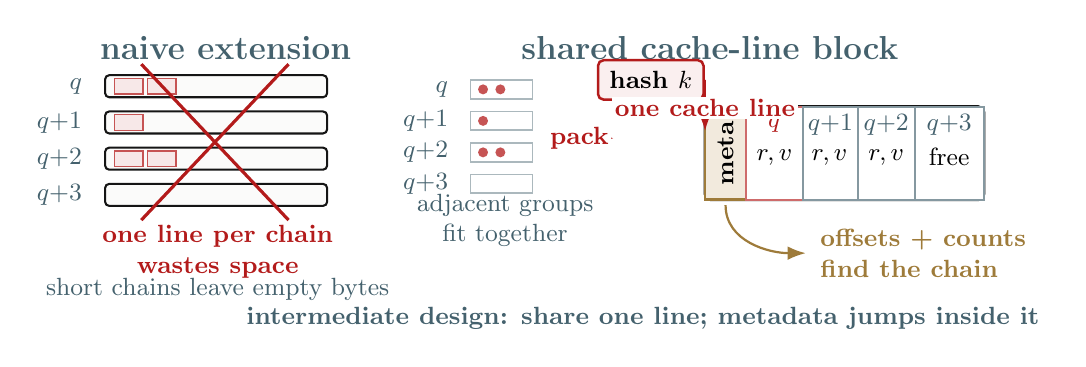
\begin{tikzpicture}[x=1cm,y=1cm,>=Latex,every node/.style={font=\large}]
    \node[font=\large\bfseries,text=BlueGray] at (-3.85,1.40) {naive extension};
    \node[font=\large\bfseries,text=BlueGray] at (2.30,1.40) {shared cache-line block};

    \foreach \y/\lab/\used in {0.92/q/2,0.46/{q{+}1}/1,0.00/{q{+}2}/2,-0.46/{q{+}3}/0} {
      \node[anchor=east,font=\small\bfseries,text=BlueGray] at (-5.55,\y) {\(\lab\)};
      \draw[Ink,line width=0.75pt,fill=CornellGray!35,rounded corners=1.5pt]
        (-5.38,\y-0.14) rectangle (-2.56,\y+0.14);
      \ifnum\used>0
        \foreach \i in {1,...,\used} {
          \draw[CornellRed!75,fill=CornellRed!10,line width=0.55pt]
            ({-5.26+0.42*(\i-1)},\y-0.10) rectangle ({-4.90+0.42*(\i-1)},\y+0.10);
        }
      \fi
    }
    \draw[CornellRed,line width=1.15pt] (-4.92,-0.78) -- (-3.05,1.20);
    \draw[CornellRed,line width=1.15pt] (-4.92,1.20) -- (-3.05,-0.78);
    \node[align=center,font=\small\bfseries,text=CornellRed] at (-3.95,-1.18)
      {one line per chain\\wastes space};
    \node[align=center,font=\small,text=BlueGray] at (-3.95,-1.66)
      {short chains leave empty bytes};

    \foreach \y/\q/\items in {0.88/q/2,0.48/{q{+}1}/1,0.08/{q{+}2}/2,-0.32/{q{+}3}/0} {
      \node[anchor=east,font=\small\bfseries,text=BlueGray] at (-0.90,\y) {\(\q\)};
      \draw[BlueGray!45,line width=0.6pt,fill=white] (-0.74,\y-0.12) rectangle (0.05,\y+0.12);
      \ifnum\items>0
        \foreach \i in {1,...,\items} {
          \fill[CornellRed!75] ({-0.58+0.22*(\i-1)},\y) circle (1.8pt);
        }
      \fi
    }
    \draw[-Latex,CornellRed,thick] (0.24,0.26) --
      node[pos=0.48,fill=white,inner sep=1pt,font=\small\bfseries,text=CornellRed] {pack} (1.08,0.26);
    \node[align=center,font=\small,text=BlueGray] at (-0.30,-0.78)
      {adjacent groups\\fit together};

    \node[draw=CornellRed,fill=CornellRed!7,line width=0.9pt,rounded corners=2pt,
          minimum width=1.34cm,minimum height=0.50cm,font=\small\bfseries] (hash) at (1.55,1.00)
      {hash \(k\)};

    \draw[Ink,line width=1.05pt,fill=CornellGray!55,rounded corners=2pt]
      (2.24,-0.52) rectangle (5.78,0.66);
    \draw[Gold!85!Ink,line width=0.85pt,fill=Gold!18]
      (2.24,-0.52) rectangle (2.76,0.66);
    \node[font=\small\bfseries,rotate=90] at (2.50,0.07) {meta};
    \foreach \xa/\xb/\lab/\col in {2.76/3.48/\(q\)/CornellRed,3.48/4.18/\(q{+}1\)/BlueGray,4.18/4.90/\(q{+}2\)/BlueGray,4.90/5.78/\(q{+}3\)/BlueGray} {
      \draw[\col!65,line width=0.7pt,fill=white] (\xa,-0.52) rectangle (\xb,0.66);
      \node[font=\small\bfseries,text=\col] at ({(\xa+\xb)/2},0.43) {\lab};
    }
    \node[font=\small] at (3.12,0.02) {\(r,v\)};
    \node[font=\small] at (3.82,0.02) {\(r,v\)};
    \node[font=\small] at (4.54,0.02) {\(r,v\)};
    \node[font=\small] at (5.34,0.02) {free};
    \draw[-Latex,CornellRed,thick] (hash.east) --
      node[pos=0.55,fill=white,inner sep=1pt,font=\small\bfseries,text=CornellRed] {one cache line} (2.24,0.35);

    \draw[-Latex,Gold!85!Ink,thick] (2.50,-0.59) to[out=-90,in=180] (3.52,-1.20);
    \node[anchor=west,align=left,text width=2.90cm,font=\small\bfseries,text=Gold!85!Ink] at (3.58,-1.20)
      {offsets + counts\\find the chain};
    \node[align=center,font=\small\bfseries,text=BlueGray] at (1.45,-2.03)
      {intermediate design: share one line; metadata jumps inside it};
  \end{tikzpicture}
  \end{center}
  \note{This slide explains the second locality opportunity. After the first tuple is moved into the head entry, the next natural question is whether we should move even more chain tuples next to the head. The naive version reserves a full cache line for every quotient chain. This would reduce chain walks, but it wastes memory badly because most chains are short; many cache lines would contain only one or two tuples and a lot of empty space. The key observation is that neighboring quotient groups are also short on average, so several adjacent groups can share one assigned cache line. The small metadata region records offsets and counts for the groups in that line. A lookup hashes to the shared line, then uses the quotient group and metadata to locate the local chain almost for free. Make clear that this is still an intermediate design idea: we are introducing the cache-line sharing intuition before the final flattened TPHT layout, not yet presenting the final home-block structure.}
\end{frame}

\begin{frame}{After Opportunity 2: What Remains?}
  \vspace{0.04cm}
  {\Large Shared cache lines help locality, but the \keyterm{overflow table can still chain}.}

  \vspace{0.10cm}
  \begin{center}
  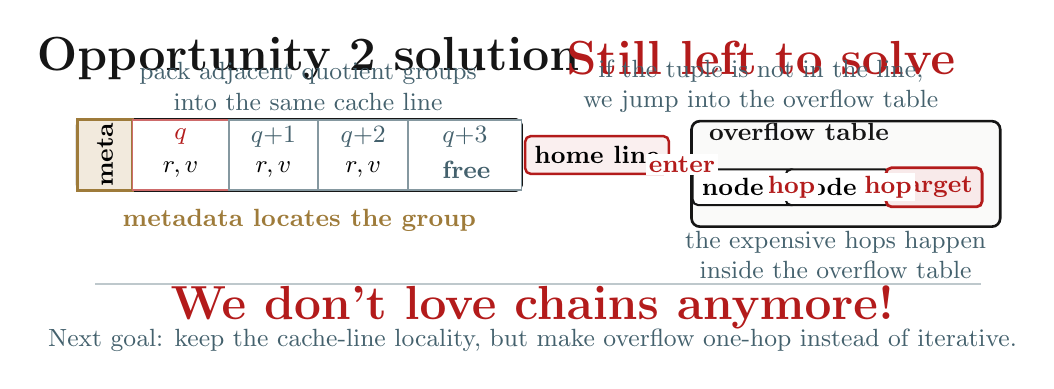
\begin{tikzpicture}[x=1cm,y=1cm,>=Latex,every node/.style={font=\large}]
    \node[font=\LARGE\bfseries,text=Ink] at (-2.85,1.72)
      {Opportunity 2 solution};
    \node[align=center,font=\small,text=BlueGray] at (-2.85,1.36)
      {pack adjacent quotient groups\\into the same cache line};

    \draw[Ink,line width=1.05pt,fill=CornellGray!55,rounded corners=2pt]
      (-5.78,0.04) rectangle (-0.14,0.94);
    \draw[Gold!85!Ink,line width=0.85pt,fill=Gold!18]
      (-5.78,0.04) rectangle (-5.08,0.94);
    \node[font=\small\bfseries,rotate=90] at (-5.43,0.49) {meta};
    \foreach \xa/\xb/\lab/\col in {-5.08/-3.86/\(q\)/CornellRed,-3.86/-2.72/\(q{+}1\)/BlueGray,-2.72/-1.58/\(q{+}2\)/BlueGray,-1.58/-0.14/\(q{+}3\)/BlueGray} {
      \draw[\col!65,line width=0.7pt,fill=white] (\xa,0.04) rectangle (\xb,0.94);
      \node[font=\small\bfseries,text=\col] at ({(\xa+\xb)/2},0.72) {\lab};
    }
    \node[font=\small\bfseries] at (-4.47,0.30) {\(r,v\)};
    \node[font=\small\bfseries] at (-3.29,0.30) {\(r,v\)};
    \node[font=\small\bfseries] at (-2.15,0.30) {\(r,v\)};
    \node[font=\small\bfseries,text=BlueGray] at (-0.84,0.30) {free};
    \node[align=center,font=\small\bfseries,text=Gold!85!Ink] at (-2.96,-0.34)
      {metadata locates the group};

    \node[font=\LARGE\bfseries,text=CornellRed] at (2.90,1.72)
      {Still left to solve};
    \node[align=center,font=\small,text=BlueGray] at (2.90,1.36)
      {if the tuple is not in the line,\\we jump into the overflow table};

    \node[draw=CornellRed,fill=CornellRed!7,line width=0.9pt,rounded corners=2pt,
          minimum width=1.35cm,minimum height=0.48cm,font=\small\bfseries] (home) at (0.82,0.49)
      {home line};
    \draw[Ink,line width=0.95pt,fill=CornellGray!45,rounded corners=3pt]
      (2.02,-0.42) rectangle (5.94,0.92);
    \node[anchor=west,font=\small\bfseries,text=Ink] at (2.12,0.78) {overflow table};
    \node[draw=Ink,fill=white,line width=0.75pt,rounded corners=2pt,
          minimum width=1.02cm,minimum height=0.40cm,font=\small\bfseries] (o1) at (2.70,0.08)
      {node 1};
    \node[draw=Ink,fill=white,line width=0.75pt,rounded corners=2pt,
          minimum width=1.02cm,minimum height=0.40cm,font=\small\bfseries] (o2) at (3.88,0.08)
      {node 2};
    \node[draw=CornellRed,fill=CornellRed!9,line width=1.0pt,rounded corners=2pt,
          minimum width=1.06cm,minimum height=0.40cm,font=\small\bfseries,text=CornellRed] (target) at (5.10,0.08)
      {target};
    \draw[-Latex,CornellRed,thick] (home.east) -- node[pos=0.55,fill=white,inner sep=1pt,font=\small\bfseries,text=CornellRed] {enter} (2.02,0.27);
    \draw[-Latex,CornellRed,thick] (o1.east) -- node[pos=0.50,fill=white,inner sep=1pt,font=\small\bfseries,text=CornellRed] {hop} (o2.west);
    \draw[-Latex,CornellRed,thick] (o2.east) -- node[pos=0.50,fill=white,inner sep=1pt,font=\small\bfseries,text=CornellRed] {hop} (target.west);
    \node[align=center,font=\small,text=BlueGray] at (3.85,-0.78)
      {the expensive hops happen\\inside the overflow table};

    \draw[BlueGray!35,line width=0.7pt] (-5.55,-1.15) -- (5.70,-1.15);
    \node[font=\LARGE\bfseries,text=CornellRed] at (0,-1.45)
      {We don't love chains anymore!};
    \node[align=center,font=\small,text=BlueGray] at (0,-1.86)
      {Next goal: keep the cache-line locality, but make overflow one-hop instead of iterative.};
  \end{tikzpicture}
  \end{center}
  \note{This slide is the breakup with chaining. First elaborate opportunity 2: rather than reserving a private cache line for every short chain, we pack adjacent quotient groups into a shared cache line and use small metadata to locate the right group. But even with this optimization, chains are still there. If the desired tuple is not in the shared line, we may still walk through overflow nodes, and every hop can cost another cache miss. Chained hash table, we had a good time. I don't love you anymore. Mark the turning point clearly: we don't love chains anymore! The next design should preserve the good cache-line packing idea, but remove iterative pointer chasing.}
\end{frame}

\begin{frame}{Flattened-TPHT: One-Hop Overflow}
  \vspace{0.04cm}
  {\Large The flattened design is a \keyterm{procedure}: fill home, then use one-hop overflow.}

  \vspace{0.08cm}
  \begin{center}
  \resizebox{0.96\textwidth}{!}{%
  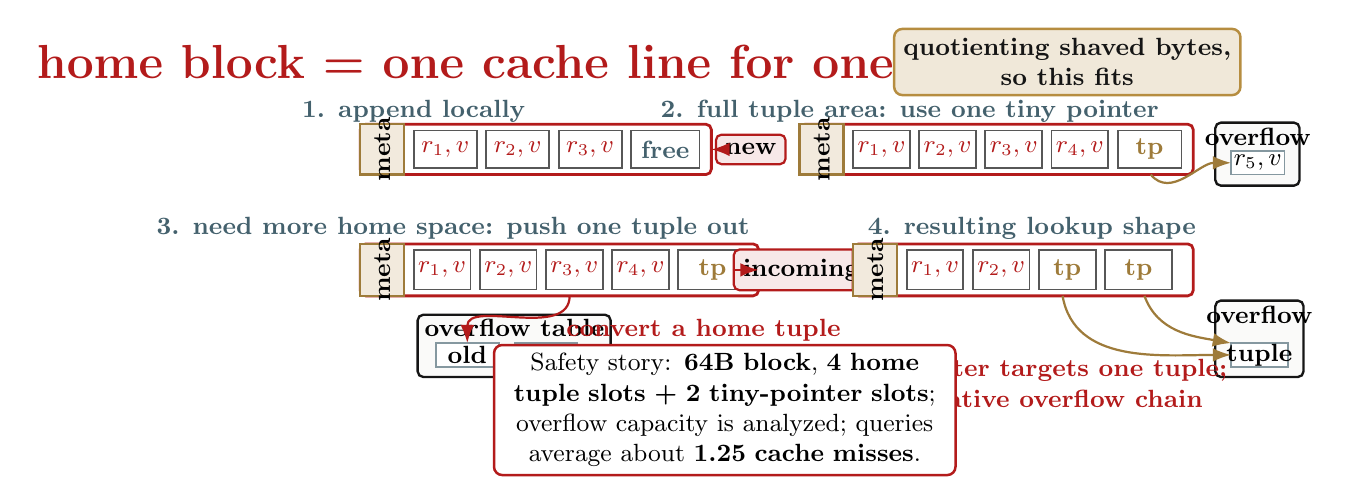
\begin{tikzpicture}[x=1cm,y=1cm,>=Latex,every node/.style={font=\large}]
    \node[font=\LARGE\bfseries,text=CornellRed] at (-3.45,2.05)
      {home block = one cache line for one bucket};
    \node[draw=Gold,fill=Gold!20,line width=0.9pt,rounded corners=3pt,
          align=center,font=\small\bfseries,text=Ink] at (3.10,2.05)
      {quotienting shaved bytes,\\so this fits};

    \node[font=\small\bfseries,text=BlueGray] at (-5.20,1.42) {1. append locally};
    \draw[CornellRed,line width=1.0pt,rounded corners=2pt]
      (-5.88,0.62) rectangle (-1.42,1.26);
    \draw[Gold!85!Ink,line width=0.85pt,fill=Gold!18]
      (-5.88,0.62) rectangle (-5.32,1.26);
    \node[font=\small\bfseries,rotate=90] at (-5.60,0.94) {meta};
    \foreach \xa/\xb/\lab/\col in {-5.20/-4.40/{\(r_1,v\)}/CornellRed,-4.28/-3.48/{\(r_2,v\)}/CornellRed,-3.36/-2.56/{\(r_3,v\)}/CornellRed,-2.44/-1.57/{free}/BlueGray} {
      \draw[Ink!72,line width=0.65pt] (\xa,0.70) rectangle (\xb,1.18);
      \node[font=\small\bfseries,text=\col] at ({(\xa+\xb)/2},0.94) {\lab};
    }
    \node[draw=CornellRed,fill=CornellRed!10,line width=0.8pt,rounded corners=2pt,
          font=\small\bfseries] (newtuple) at (-0.92,0.94) {new};
    \draw[-Latex,CornellRed,thick] (newtuple.west) -- (-1.42,0.94);

    \node[font=\small\bfseries,text=BlueGray] at (1.10,1.42) {2. full tuple area: use one tiny pointer};
    \draw[CornellRed,line width=1.0pt,rounded corners=2pt]
      (-0.30,0.62) rectangle (4.70,1.26);
    \draw[Gold!85!Ink,line width=0.85pt,fill=Gold!18]
      (-0.30,0.62) rectangle (0.26,1.26);
    \node[font=\small\bfseries,rotate=90] at (-0.02,0.94) {meta};
    \foreach \xa/\xb/\lab/\col in {0.38/1.10/{\(r_1,v\)}/CornellRed,1.22/1.94/{\(r_2,v\)}/CornellRed,2.06/2.78/{\(r_3,v\)}/CornellRed,2.90/3.62/{\(r_4,v\)}/CornellRed,3.74/4.55/{tp}/Gold!85!Ink} {
      \draw[Ink!72,line width=0.65pt] (\xa,0.70) rectangle (\xb,1.18);
      \node[font=\small\bfseries,text=\col] at ({(\xa+\xb)/2},0.94) {\lab};
    }
    \draw[Ink,line width=0.85pt,fill=CornellGray!40,rounded corners=2pt]
      (4.98,0.48) rectangle (6.05,1.28);
    \node[font=\small\bfseries] at (5.52,1.10) {overflow};
    \draw[BlueGray!65,line width=0.6pt,fill=white] (5.18,0.62) rectangle (5.86,0.92);
    \node[font=\small\bfseries] at (5.52,0.77) {\(r_5,v\)};
    \draw[-Latex,Gold!85!Ink,thick] (4.16,0.62) to[out=-50,in=180] (5.18,0.77);

    \node[font=\small\bfseries,text=BlueGray] at (-4.70,-0.06) {3. need more home space: push one tuple out};
    \draw[CornellRed,line width=1.0pt,rounded corners=2pt]
      (-5.88,-0.92) rectangle (-0.82,-0.26);
    \draw[Gold!85!Ink,line width=0.85pt,fill=Gold!18]
      (-5.88,-0.92) rectangle (-5.32,-0.26);
    \node[font=\small\bfseries,rotate=90] at (-5.60,-0.59) {meta};
    \foreach \xa/\xb/\lab/\col in {-5.20/-4.48/{\(r_1,v\)}/CornellRed,-4.36/-3.64/{\(r_2,v\)}/CornellRed,-3.52/-2.80/{\(r_3,v\)}/CornellRed,-2.68/-1.96/{\(r_4,v\)}/CornellRed,-1.84/-0.97/{tp}/Gold!85!Ink} {
      \draw[Ink!72,line width=0.65pt] (\xa,-0.84) rectangle (\xb,-0.34);
      \node[font=\small\bfseries,text=\col] at ({(\xa+\xb)/2},-0.59) {\lab};
    }
    \node[draw=CornellRed,fill=CornellRed!10,line width=0.8pt,rounded corners=2pt,
          font=\small\bfseries] (incoming) at (-0.28,-0.59) {incoming};
    \draw[-Latex,CornellRed,thick] (incoming.west) -- (-0.82,-0.59);
    \draw[Ink,line width=0.85pt,fill=CornellGray!40,rounded corners=2pt]
      (-5.15,-1.95) rectangle (-2.70,-1.16);
    \node[font=\small\bfseries] at (-3.92,-1.32) {overflow table};
    \draw[BlueGray!65,line width=0.6pt,fill=white] (-4.92,-1.82) rectangle (-4.12,-1.52);
    \draw[BlueGray!65,line width=0.6pt,fill=white] (-3.92,-1.82) rectangle (-3.12,-1.52);
    \node[font=\small\bfseries] at (-4.52,-1.67) {old};
    \node[font=\small\bfseries] at (-3.52,-1.67) {new};
    \draw[-Latex,CornellRed,thick] (-3.22,-0.92) to[out=-90,in=90] (-4.52,-1.52);
    \node[align=center,font=\small\bfseries,text=CornellRed] at (-1.52,-1.55)
      {convert a home tuple\\into a tiny pointer};

    \node[font=\small\bfseries,text=BlueGray] at (2.65,-0.06) {4. resulting lookup shape};
    \draw[CornellRed,line width=1.0pt,rounded corners=2pt]
      (0.38,-0.92) rectangle (4.70,-0.26);
    \draw[Gold!85!Ink,line width=0.85pt,fill=Gold!18]
      (0.38,-0.92) rectangle (0.94,-0.26);
    \node[font=\small\bfseries,rotate=90] at (0.66,-0.59) {meta};
    \foreach \xa/\xb/\lab/\col in {1.06/1.78/{\(r_1,v\)}/CornellRed,1.90/2.62/{\(r_2,v\)}/CornellRed,2.74/3.46/{tp}/Gold!85!Ink,3.58/4.43/{tp}/Gold!85!Ink} {
      \draw[Ink!72,line width=0.65pt] (\xa,-0.84) rectangle (\xb,-0.34);
      \node[font=\small\bfseries,text=\col] at ({(\xa+\xb)/2},-0.59) {\lab};
    }
    \draw[Ink,line width=0.85pt,fill=CornellGray!40,rounded corners=2pt]
      (4.98,-1.95) rectangle (6.10,-0.98);
    \node[font=\small\bfseries] at (5.54,-1.16) {overflow};
    \draw[BlueGray!65,line width=0.6pt,fill=white] (5.18,-1.82) rectangle (5.90,-1.52);
    \node[font=\small\bfseries] at (5.54,-1.67) {tuple};
    \draw[-Latex,Gold!85!Ink,thick] (3.04,-0.92) to[out=-80,in=180] (5.18,-1.67);
    \draw[-Latex,Gold!85!Ink,thick] (4.08,-0.92) to[out=-70,in=170] (5.18,-1.52);
    \node[align=center,font=\small\bfseries,text=CornellRed] at (2.65,-2.03)
      {tiny pointer targets one tuple;\\no iterative overflow chain};

    \node[draw=CornellRed,fill=white,line width=0.9pt,rounded corners=3pt,
          align=center,text width=5.65cm,font=\small,inner sep=3pt] at (-1.25,-2.37)
      {Safety story: \textbf{64B block}, \textbf{4 home tuple slots + 2 tiny-pointer slots}; overflow capacity is analyzed; queries average about \textbf{1.25 cache misses}.};
  \end{tikzpicture}
  }
  \end{center}
  \note{This slide introduces Flattened-TPHT in a simplified way for the audience. We do not need to exactly follow every construction detail from the paper. The story is: each key bucket owns a cache-line home block. We append quotient-compressed tuples into the home block first. If we cannot append a full tuple, we store a tiny pointer to one tuple in the overflow table. Stress that this is not a linked list: the overflow tuple does not iteratively point to more overflow tuples. If more room is needed in the home block, we can push one existing tuple to the overflow table and replace it by a tiny pointer, which creates more space for new home-resident tuples or more tiny pointers. This works because quotienting shaved bytes off the stored keys. If the audience asks whether four home slots, two pointer slots, and the overflow table are enough, say that the paper analyzes these capacity questions and sizes the overflow pool using the spill tail; the slide gives the key numbers and the measured result that queries average about 1.25 cache misses.}
\end{frame}

\begin{frame}{Transition: Experimental Results}
  \vspace{-0.08cm}
  \begin{center}
    {\LARGE\bfseries Do tiny pointers survive a systems benchmark?}\par
    \vspace{0.03cm}
    {\large\color{BlueGray} We evaluate both TPHT variants under the same conditions as strong production-style hash tables.}
  \end{center}

  \vspace{-0.04cm}
  \begin{columns}[T,onlytextwidth]
    \column{0.32\textwidth}
      \begin{block}{Machine}
        \small
        \textbf{Single-socket server}\par
        Intel Xeon Silver 4314\par
        16 cores / 32 threads\par
        128 GiB RAM, 24 MiB L3\par
        Linux 5.15, one NUMA node
      \end{block}
    \column{0.32\textwidth}
      \begin{block}{Workloads}
        \small
        \textbf{64-bit keys + values}\par
        YCSB hash-table variant\par
        load: 64M inserts\par
        runs: A/B/C, negative queries, deletes\par
        plus uniform-key microbenchmarks
      \end{block}
    \column{0.32\textwidth}
      \begin{block}{Comparisons}
        \small
        libcuckoo, IcebergHT, Junction, TBB\par
        compact tables: bucketing, Cleary, Layered\par
        throughput, space efficiency, scaling, resizing\par
        no duplicate keys in benchmarks
      \end{block}
  \end{columns}

  \vspace{0.02cm}
  \begin{center}
  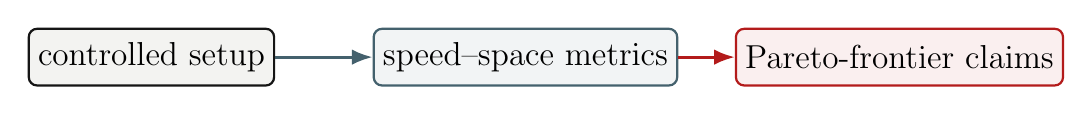
\begin{tikzpicture}[x=1cm,y=1cm,every node/.style={font=\large}]
    \node[draw=Ink,fill=CornellGray,rounded corners=3pt,line width=0.8pt,minimum width=3.10cm,minimum height=0.72cm] (setup) at (-4.75,0) {controlled setup};
    \node[draw=BlueGray,fill=BlueGray!7,rounded corners=3pt,line width=0.8pt,minimum width=3.10cm,minimum height=0.72cm] (metrics) at (0,0) {speed--space metrics};
    \node[draw=CornellRed,fill=CornellRed!7,rounded corners=3pt,line width=0.8pt,minimum width=3.10cm,minimum height=0.72cm] (claims) at (4.75,0) {Pareto-frontier claims};
    \draw[-Latex,line width=1pt,BlueGray] (setup.east) -- (metrics.west);
    \draw[-Latex,line width=1pt,CornellRed] (metrics.east) -- (claims.west);
  \end{tikzpicture}
  \end{center}

  \vspace{-0.04cm}
  \centering
  {\large\textbf{Space efficiency} = raw key--value payload / maximum allocated memory footprint.}
\end{frame}

\begin{frame}{Result: TPHT Moves the Space Frontier}
  \vspace{-0.04cm}
  \begin{columns}[T,onlytextwidth]
    \column{0.52\textwidth}
      \begin{center}
      {\small\bfseries Figure 1(a): YCSB throughput}\\[-0.08cm]
      \begin{tikzpicture}
        \begin{axis}[
          ybar,
          width=\linewidth,
          height=0.55\textheight,
          ymin=0,
          ymax=430,
          ylabel={throughput (M ops/s)},
          ylabel style={font=\small},
          symbolic x coords={Cuckoo,Iceberg,Junction,TBB,Chained,Flattened},
          xtick={Cuckoo,Iceberg,Junction,TBB,Chained,Flattened},
          x tick label style={rotate=28,anchor=east,font=\small},
          y tick label style={font=\small},
          legend style={draw=none,fill=none,at={(0.50,1.03)},anchor=south,legend columns=2,font=\small},
          bar width=4.3pt,
          enlarge x limits=0.11,
          axis line style={draw=Ink},
          grid=major,
          grid style={CornellGray},
          major grid style={line width=0.25pt,draw=CornellGray},
          tick align=outside
        ]
          \addplot[fill=BlueGray!48,draw=BlueGray] coordinates
            {(Cuckoo,116.1) (Iceberg,114.3) (Junction,18.4) (TBB,8.5) (Chained,100.4) (Flattened,227.5)};
          \addplot[fill=CornellRed!74,draw=CornellRed] coordinates
            {(Cuckoo,130.5) (Iceberg,167.5) (Junction,156.7) (TBB,40.2) (Chained,196.0) (Flattened,391.2)};
          \legend{load, run}
        \end{axis}
      \end{tikzpicture}
      \end{center}
    \column{0.45\textwidth}
      \begin{center}
      {\small\bfseries Figure 1(b): max space efficiency}\\[-0.08cm]
      \begin{tikzpicture}
        \begin{axis}[
          ybar,
          width=\linewidth,
          height=0.55\textheight,
          ymin=0,
          ymax=120,
          ylabel={space efficiency (\%)},
          ylabel style={font=\small},
          symbolic x coords={TBB,Cuckoo,Junction,IcebergHT,Flattened,Chained},
          xtick={TBB,Cuckoo,Junction,IcebergHT,Flattened,Chained},
          x tick label style={rotate=28,anchor=east,font=\small},
          y tick label style={font=\small},
          nodes near coords,
          nodes near coords style={font=\small,anchor=south},
          bar width=7pt,
          enlarge x limits=0.12,
          axis line style={draw=Ink},
          grid=major,
          grid style={CornellGray},
          major grid style={line width=0.25pt,draw=CornellGray},
          tick align=outside
        ]
          \addplot[fill=BlueGray!48,draw=BlueGray] coordinates
            {(TBB,32.3) (Cuckoo,70.1) (Junction,75.0) (IcebergHT,81.7)};
          \addplot[fill=CornellRed!78,draw=CornellRed] coordinates
            {(Flattened,83.4) (Chained,105.4)};
        \end{axis}
      \end{tikzpicture}
      \end{center}
  \end{columns}
  \vspace{0.02cm}
  \centering
  {\large Chained-TPHT goes beyond the raw key-value payload size; Flattened-TPHT is both compact and fast.}
\end{frame}

\begin{frame}{Figure 8(a): Insertion Throughput vs. Space}
  \vspace{-0.08cm}
  \begin{center}
  \begin{tikzpicture}
    \begin{axis}[
      width=0.91\linewidth,
      height=0.62\textheight,
      xmin=0,
      xmax=110,
      ymin=0,
      ymax=27,
      xlabel={space efficiency (\%)},
      ylabel={insertion throughput (M ops/s)},
      xlabel style={font=\small},
      ylabel style={font=\small},
      tick label style={font=\small},
      axis line style={draw=Ink},
      grid=major,
      major grid style={line width=0.25pt,draw=CornellGray},
      minor tick num=1,
      legend style={draw=none,fill=none,at={(0.5,1.04)},anchor=south,legend columns=3,font=\small},
      legend cell align=left,
      every axis plot/.append style={line width=1.05pt,mark size=1.65pt},
    ]
      \addplot[color=BlueGray!72!Ink,mark=o] coordinates {(4.4,11.3) (8.8,10.8) (13.2,10.4) (17.5,10.1) (21.9,9.8) (26.3,9.5) (30.7,9.3) (35.1,9.0) (39.5,8.7) (43.8,8.3) (48.2,7.9) (52.6,7.5) (57.0,7.0) (61.4,6.5) (65.8,6.0) (70.1,5.3)};
      \addplot[color=Gold!92!Ink,mark=square*] coordinates {(4.1,15.2) (8.3,15.9) (12.4,16.3) (16.5,16.4) (20.6,16.2) (24.8,16.2) (28.9,16.1) (33.0,15.9) (37.1,15.8) (41.3,15.7) (45.4,15.5) (49.5,15.4) (53.6,15.2) (57.8,15.1) (61.9,14.9) (66.0,14.8) (70.1,14.6) (74.3,14.4) (78.4,14.3) (81.7,14.0)};
      \addplot[color=Green!88!Ink,mark=triangle*] coordinates {(5.0,19.1) (10.0,20.2) (15.0,20.0) (20.0,19.7) (25.0,19.5) (30.0,19.1) (35.0,18.8) (40.0,18.3) (45.0,18.0) (50.0,17.5) (55.0,17.1) (60.0,16.5) (65.0,15.9) (70.0,15.3) (75.0,14.6)};
      \addplot[color=Purple!88!Ink,mark=diamond*] coordinates {(6.2,2.6) (10.0,2.6) (13.1,2.7) (15.6,2.7) (17.1,2.8) (19.9,2.8) (20.8,2.9) (22.3,2.9) (23.3,3.0) (24.7,3.0) (25.4,3.0) (27.1,3.1) (27.6,3.0) (28.6,3.1) (29.1,3.1) (29.3,3.2) (30.5,3.2) (30.9,3.2) (31.2,3.2) (32.3,3.2)};
      \addplot[color=CornellRed!86!Ink,mark=*,line width=1.25pt] coordinates {(5.3,12.9) (10.6,13.0) (16.0,12.9) (21.3,12.7) (26.6,12.4) (31.9,12.1) (37.3,11.8) (42.6,11.4) (47.9,11.2) (53.2,10.9) (58.6,10.6) (63.9,10.3) (69.2,10.0) (74.5,9.8) (79.9,9.5) (85.2,9.3) (90.5,9.1) (95.8,8.9) (101.2,8.7) (105.4,8.5)};
      \addplot[color=CornellRed!62!Gold,mark=pentagon*,line width=1.25pt] coordinates {(4.2,24.7) (8.4,24.5) (12.6,24.6) (16.8,24.5) (21.1,24.1) (25.3,23.9) (29.5,23.7) (33.7,23.5) (37.9,23.2) (42.1,22.8) (46.3,22.6) (50.5,22.2) (54.8,21.9) (59.0,21.5) (63.2,20.9) (67.4,20.7) (71.6,20.3) (75.8,19.9) (80.0,19.3) (83.4,19.0)};
      \draw[dashed,CornellRed!65,line width=0.7pt] (axis cs:100,0) -- (axis cs:100,27);
      \node[anchor=south east,font=\small,text=CornellRed] at (axis cs:99.2,0.6) {100\% payload};
      \legend{Cuckoo, IcebergHT, Junction, TBB, Chained-TPHT, Flattened-TPHT}
    \end{axis}
  \end{tikzpicture}
  \end{center}
  \vspace{-0.02cm}
  \centering
  {\large Each curve sweeps load factor; TPHT pushes farther right while keeping competitive insertion throughput.}
\end{frame}

\begin{frame}{Summary: What TPHT Delivers}
  \vspace{0.04cm}
  \begin{center}
    {\Large Tiny pointers turn a few saved key bits into a better speed--space tradeoff.}
  \end{center}

  \vspace{0.18cm}
  \begin{columns}[T,onlytextwidth]
    \column{0.31\textwidth}
      \begin{block}{Compactness}
        \small
        \metric{105.4\%}{max space efficiency}\par
        \vspace{0.08cm}
        \Chained stores less than the raw key--value payload by using quotient bits and tiny-pointer chains.
      \end{block}
    \column{0.31\textwidth}
      \begin{block}{Throughput}
        \small
        \metric{391.2M}{avg run-phase ops/s}\par
        \vspace{0.08cm}
        \Flat is the fastest YCSB design while keeping higher space efficiency than the baselines.
      \end{block}
    \column{0.31\textwidth}
      \begin{block}{Pareto frontier}
        \small
        \metric{83.4\%}{\Flat space efficiency}\par
        \vspace{0.08cm}
        Across load factors, TPHT reaches farther right without giving up competitive insertion throughput.
      \end{block}
  \end{columns}

  \vspace{0.20cm}
  \begin{center}
  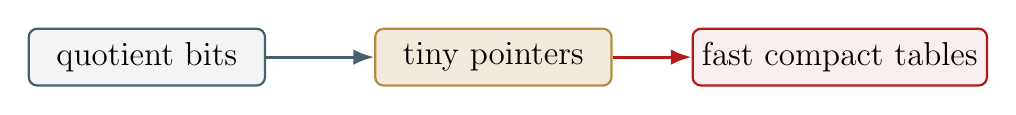
\begin{tikzpicture}[x=1cm,y=1cm,every node/.style={font=\large}]
    \node[draw=BlueGray,fill=BlueGray!7,rounded corners=3pt,line width=0.8pt,minimum width=3.0cm,minimum height=0.72cm] (bits) at (-4.4,0) {quotient bits};
    \node[draw=Gold,fill=Gold!18,rounded corners=3pt,line width=0.8pt,minimum width=3.0cm,minimum height=0.72cm] (ptrs) at (0,0) {tiny pointers};
    \node[draw=CornellRed,fill=CornellRed!7,rounded corners=3pt,line width=0.8pt,minimum width=3.0cm,minimum height=0.72cm] (tables) at (4.4,0) {fast compact tables};
    \draw[-Latex,line width=1pt,BlueGray] (bits.east) -- (ptrs.west);
    \draw[-Latex,line width=1pt,CornellRed] (ptrs.east) -- (tables.west);
  \end{tikzpicture}
  \end{center}

  \vspace{0.12cm}
  \centering
  {\small The main lesson: succinct hashing ideas can be engineered into practical, concurrent hash tables.}
\end{frame}

\begin{frame}[plain]
  \titleband
  \vspace{1.5cm}
  \begin{beamercolorbox}[wd=0.82\paperwidth,sep=0.35cm,left]{title}
    \usebeamerfont{title}Thank you.\par
    \vspace{0.2cm}
    {\Large Questions?}
  \end{beamercolorbox}
  \vspace{0.45cm}
  \begin{beamercolorbox}[wd=0.82\paperwidth,sep=0.35cm,left]{author}
    \small Xilin Tang \quad Cornell University\par
    \vspace{0.2cm}
    \small Artifact: \texttt{github.com/Xilinion/TinyPtr}
  \end{beamercolorbox}
\end{frame}

\end{document}
